\documentclass[letterpaper, 12 pt]{article}
\usepackage[left=2.0cm,top=2.5cm,right=2.0cm,bottom=2.5cm,bindingoffset=0.5cm]{geometry}
\usepackage{appendix}
\usepackage{listings}
\usepackage{verbatim}
\usepackage{minted}
\usepackage{graphicx}
\usepackage{pdfpages}
\usepackage{float}
\usepackage{hyperref}


\title{\Huge \textbf{LifeSense}} 
\author{Zach Toolson and Dan Willoughby }

\begin{document}
\maketitle
\clearpage

\tableofcontents
\clearpage

\section{Introduction}
Life is full of unexpected surprises. Some days you can come home and find you left the lights on wasting your hard earned cash on an electricity bill. Other days you might find that your dog is laying on your couch, even though you told it not to. So much for those dog treats you used when you thought it was being a good dog. Probably the worst unexpected surprise though, is when you have already poured your favorite cereal only to find that there is not any milk left in the fridge.

The problem that our project solves is providing a way for people to monitor data from their lives and interact with it in a meaningful way. In other words, it helps lessen the unexpectedness of those unexpected surprises. Our project provides a way for you to turn off your lights from anywhere, even after you have left your house (if your house is super small and lit with LEDs). You can detect when that dog jumps up on the couch and be notified via email when it does. You can track the amount of milk left in your fridge based off its weight and check its levels in real-time. Thats right, you can see how much milk is in your fridge in real-time! No more missing out on your favorite cereal. 

On a more serious note, our project is a platform for managing sensors and controlling peripherals. Our project involves a printed circuit board (PCB) with wireless network capabilities that we designed, fabricated, and soldered. Since the PCB is wireless it can be placed anywhere, so that data can be gathered in anyplace without having to run a wire to a central control station. Our project provides a complete and functional website to manage multiple PCBs in one place. The website allows users to see a history of sensor data, view real-time updates, get email notifications, configure PCBs, and control peripherals, all from the comfort of a laptop or smartphone. Although its not quite ready to be stocked on Home Depot’s selves, its functionality is complete enough for any electronic hobbyists that is interested in managing sensors and controlling peripherals via wifi. 

\section{Background}
The background of our project comes from Dan wanting to keep track how much milk he had left in the milk carton in his fridge, and receive an email when the milk was almost gone. We both thought it would be a pretty cool thing to have so we started work on the project in our Embedded Systems class. After we built a prototype in Embedded Systems, we decided to continue working on it for our senior project. We realized that we could expand on the simple prototype we made for simply tracking milk, into a project that would work with any sensor and could be used from any device with a web browser. 

Another huge contributor to the decision on our project was we wanted to make something useful. We actually wanted to use the project that we were making, if not to track milk, but to track motion, temperature, or weight. We laid the foundation to work on something we were passionate about and set a goal for the project to have an awesome demo. From the very beginning of the project, we envisioned people on demo day sincerely saying "Wow! That’s cool!", instead of people purposely lying and saying "Ohh... looks great guys." 

Planning began the beginning of 2014 and continued for about 4 months. Although we had a general idea of what we wanted to do, the project really evolved over the summer and in the fall when we started implementing our ideas. We adjusted our plans and even made new ones. 

\section{Project Implementation}

\subsection{Printed Circuit Board}
Our printed circuit board (PCB) handled most of the input from the sensors and controlled outputs such as LEDs. The PCB needed to have a way to communicate wirelessly and have a powerful enough microcontroller in order to interface with the network processor. We decided to use the Cortex M4 microcontroller and the CC3000 network processor. The main reason for the Cortex M4 was because we had previous experience with it and it was a relatively popular chip. We also owned a Stellaris Launchpad  from TI which featured the Cortex M4. We decided to use the CC3000 in our Embedded Systems class. During the class, we made a prototype PCB which just had the CC3000 soldered onto it. We connected the CC3000 with several wires to the Stellaris Launchpad and we were surprised, but relieved when it was fetching data from a website. In terms of first motivating successes, fetching data for the first time with the prototype was one of the firsts. The remainder of our time in Embedded Systems we worked on creating a prototype that was able to collect data from a scale and display it on a very simple website. 
  
  The actual creation of the PCB for our senior project was never really planned nor even thought possible. During the spring semester, we never officially decided to fabricate a PCB, but it all started when we found a schematic of the stellaris launchpad and started looking at the data sheet for the CC3000. After some time of studying the schematic, it seemed more of a possibility, but never something we’d actually try. We heard from a friend that Kicad was a cool open source tool that was pretty similar to Altium. Since we had fabricated a PCB in Embedded Systems and thought it was cool that we made a board that worked in that class, we decided to learn how Kicad worked. We followed a youtube video series that taught the basics of Kicad and for awhile that’s as far as we thought it’d go. 

  One day, we just started looking up footprints on the internet for the parts of the prototype. After finding the footprints for the Cortex M4 and CC3000, as a joke we decided to place both the footprints in a project, just to see how insane it would be to connect the 64 pin microcontroller to a 30 or so pin network processor. Progress on the PCB continued in this way for awhile, just for fun we’d add some more components like capacitors or resistors and joke around saying, man we’d be nuts to actually connect all these footprints and pins together with traces. Shortly after the fall semester started, we just decided to do it. We said to ourselves, well if the PCB does not work we can just use the prototype, what do we have to lose? We spent about a week finalizing the design (connecting each of the 64 pins on the microcontroller, which took forever), creating some of our own footprints, and determined which parts we’d need to order. 

    The first run of the board did not work completely, but it was successful in some ways. We figured out that our micro-usb footprint was too big and that we had wired up our LEDs backwards. If that had been our only mistake the board might have been usable, but we forgot to connect 4 pins to each other on the CC3000 so we had no networking abilities at all. After we discovered those issues we quickly fixed them and order the second board. The second order or boards in roughly two weeks. At this time we calculated if the board did not work, we had roughly 2 or 3 more tries to get it to work before we were out of time. We were hopeful it would work, but still in the back of our minds we thought “how could it possibly work, its such a complicated board.” After it was soldered, we loaded on some sample code and the board worked (details later about what worked means)! It was an awesome feeling. Looking back we were really happy with the decision to make the board. It really enhanced the project and gave it the cool factor. 
      
      After we had the boards complete we were able to focus more on the software side of the project. We named the Embedded devices, transmitters. The name was fitting and allowed for the details of the embedded device to be abstracted away from the user and allow it to be configured more easily on the website.  

\subsection{Ruby on Rails}
Ruby on Rails served as the backend of project that kept track of our data and served up our website. Rails is a modern web framework used to create dynamic web pages that is open source and written in the Ruby language. We were both familiar with Rails and we both wanted to get better at developing applications with it. It seemed like the logical choice for our website. Even though Rails did not have anything that was visual for the user to see (such as a GUI), it was extremely important to the success of our project.

  Rails made it easy to keep track of all the dynamic information and data. The Rails framework abstracts the tricky details of a database (such as migrations, tables, and columns) and maps database entries to objects. The bonus was that we could create objects by receiving information from the user, manipulate the objects if needed, and then save the information into the database, all within a single line of code (and not just one really long line of code, in under 5 words). 

  We saved a lot of data in our database. Information about user accounts, sensor data that was collected, and  information for the setup of transmitters and sensors. The user login information allowed our website to serve many different users. Each user could create transmitters and sensors and configure them so that they were associated with each other. For example, you could create a transmitter called LIfeSense which had about 20 pin numbers. The user could then create a sensor and assign it to the LifeSense transmitter and a pin number belonging to that transmitter. At a later time, if they moved the sensor to a different transmitter, all that was required was reassigning the transmitter and pin number on the website. The user did not have to reprogram their Embedded Device which is a feature we were quite proud of. 

  The dynamic functionality of switching sensors between transmitters came at a cost, however. We needed a way to determine which transmitter data was coming from. Our solution was to assign a token to each transmitter that the user would program into the PCB software. Each time the transmitter posted data to the website it would include its token and which pin number the data belonged to. From there we could do a reverse lookup to find the right sensor. To find the sensor, we first found the transmitter object based off its token. A transmitter could list all its pin numbers, so from there we could select the pin number and create a record of the data for the sensor.

  The last piece of the puzzle was getting data from the Rails server to our website. We decided fairly early on in our project that we wanted to make an API so that all our data could be updated, created, deleted, or read from JSON requests. JSON is a convention for specifying data structures in text, so for instance an array would be declared as an open and close bracket with commas separating values and a dictionary or hash would be similar, but use curly braces instead. The main reason for making an API was so we could make smartphone applications (if we had time), but it turned out it made it easier for using a rich user interface javascript framework.  

  We chose to use Ruby on Rails because it is optimized for programmers happiness and productivity. Rails uses a model, view, controller model which separates concerns and provides a very logical pattern of developing a web server. Rails also has a thriving community that allowed us to use ‘gems’, or modules that are written by other programmers very easily. One example of this is using the ‘denkatu’ gem which was a simple library that provided calculator functionality to apply the sensor’s formula (which was usually a polynomial) to data coming in. Rails was very helpful in the storage of our data, but we found it lacking in its ability to create a responsive front-end user interface. 

\subsection{Ember}
Ember was the front end of the project that was most of what the user saw, but it was not part of our original plan. We had absolutely no experience with Ember when we decided to use it, but we had a major dilemma. We had spent a month or so implementing a Rails website and all we had been able to create was a website that could track time. It was just overly frustrating to have Rails function as the user interface for dynamically changing content. Our time-tracker was slow and severely lacked functionality and the time tracker was not even a main feature of the project, it was just supposed to be something simple. At about the same time we finished the time tracker in Rails we heard about Ember. Ember.js is a javascript framework used for creating ambitious web applications and follows a lot of the same conventions and ideas as the Ruby on Rails framework. We made the decision to invest the time to learn a new framework, since we had already had some success with our PCB.

  Learning Ember took way longer than expected. We spent several weeks following multiple tutorials. Some times we thought we had made the wrong decision switching, especially since we were already a month into development and time was running out. 

  Our decision paid off after a while as we started to get a hand of the frame work. It allowed us to have formula’s to change sensor’s data on the fly as it displayed in graphs. It helped us in implementing a simple yet intuitive interface for sensors and transmitters. The best part was it provided a local mapping our server data, handling requests to Rails, caching results, and updates, all with little effort on our part. Ember allowed us to integrate with the highcharts graphing library for Javascript allowing our users to view live graphs, and detailed graphs of historical data that they could drag and zoom in on data points. We were able to add animated switches for users to flip on and off LEDs. We owe a lot of the simplistic nature of our website to Ember and a lot of the dynamic functionality that came with it. 


\subsection{Node}
Node was used to tie everything together. We had the Rails server to store all our data, an Embedded Device to collect data, Ember to display and collect data from the user, but we needed some way to get all these pieces together. We had a simple solution, that required the user to press refresh a lot to see updated data, or to wait quite a while for LEDs to turn on or off. We were at a point where we were almost decided to be content with the simple solution. It was then we thought back to our initial goal of our project. We wanted a sincere, "Wow! That’s cool" instead of "Ohh... looks great guys."  So we pressed on with a more complicated solution that would allow for the communication between each piece of our project to be real-time. We just knew the real-time functionality would really give the wow factor we were looking for.  

 Node.js is a web development framework has great functionality for concurrent connections, so it seemed like the perfect fit for our live communication. We also had some previous experience with node when we made our prototype in the spring so that helped in making the decision. Our alternative was using some gems in Rails, but we quickly became frustrated by the options Rails had available. 

  The node server was pretty basic in concept but more difficult in implementation. Node kept a connection alive with each transmitter and continuously fetched data from them. We used the http protocol to send requests and responses. The transmitter read its sensor data and posted it to the node server. The node server would then respond in json with the values that the outputs should be. So for example, if pin A0 was an input and pin A1 was an output on the embedded device, every second the embedded device would read pin A0 and send in that value. Then node would tell the embedded device to set pin A1 to high in its response. We implemented the communication this way because it used existing functionality in both node and the embedded device’s software libraries.

    The other function of the node server was communicating live data to and from the Ember apps. The idea was to have the user see live data points on a graph as it was being read from a sensor, or be able to flip a switch on the web browser and have it turn off an LED instantly. In order to achive the functionality, we used a library called socket.io to keep a web socket open. We had some previous experience implementing sockets so it was relatively easy to implement once we got the some socket.io libraries working. After the sockets connected, the node server could send out the embedded device data based on its token. The web browser or Ember app could then parse the data for the correct graph (again based on the transmitters token) and display it to the user. The LEDs worked in a similar way, when a user flipped the switch, the web browser sent a message with the transmitter token and pin number to node, then node would tell the appropriate device to turn on/off that LED. 

    The live data part of our project was an unplanned, but an added bonus. We left it till the very end, because we knew it added additional complexity. We knew though, however, without real-time data, the project would be kind of lame, so we worked hard to make it functional with just a few days to spare before demo day.  

\section{Evaluation}

\subsection{Printed Circuit Board}
We were very happy with our PCB and felt very lucky that it worked. In simplest terms, the PCB did everything we wanted it to. It connected the WiFi, it collected data from sensors, it controlled peripherals, and it was able to be controlled over the WiFi connection. The main tests we did on the PCB was to see how long a connection could stay alive. We found that if the PCB acted as its own web server, the connection would die quickly, but if it was constantly posting data and receiving responses the connection would last a long time. Our longest period of posting and receiving responses was 13 hours  and even then we manually stopped the board to move it. 

  We had a PCB stop working the day before the demo. Luckily, we had a spare board so we were able to replace it. It was pretty scarey when the board would not connect to WiFi, it was as if our CC3000 completely died. Another thing we noticed was some of the GPIOs did not work very well, but since we had wired up some many of them initially we had plenty left over for our demo. 

\subsection{Ruby on Rails}
Ruby on Rails worked great as a web server that would communicate between the front end Ember.js application and our database. Some of the difficulties that we had using Ruby on Rails were getting the emails to be sent from our local machines. Many web tutorials all pointed to the same way of sending emails, but didn’t work. What was required is installing a SMTP server on our local machines to send the email for Ruby on Rails. Another thing that was questionable is that our Ruby on Rails formula evaluating library would evaluate the values slightly differently than the javascript library that we were using on the front end, which caused some irregularities in the email when checking if a value is above or below a certain value. Our testing strategy was mostly using the command line tool curl to verify that the proper data was being served up in JSON format and records, sensors, and transmitters would be saved properly.

\subsection{Ember}
Ember was a love hate relationship. Even though it provided great tools for fetching and receiving data from our Rails backend, we just had constant headaches when implementing things that were not natively supported. One frustration was updating relationships between pin numbers and sensors. Ember did not provide a way to detect when a relationship had changed, so we had to manually do it ourselves. Another thing was applying the user token in the HTTP headers so that our Rails server would see our JSON request as authenticated. We eventually came up with some hacked together solutions, but each hacked solution cost us tons of time and effort. 

Since a majority of our Ember code was for User interface, we simply clicked around on the website to determine the functionality we expect was there. 

\subsection{Node}
Node was perhaps the fastest development for our project. Every aspect went fast and smooth. Node provided all the tools we needed to communicate our real-time data between our Ember app, embedded devices, and our Rails backend. To the credit of all the other frameworks we used, Node had the simplest job to do, so that contributed to the good experience we had. 

\section{Conclusion}
The goal of our final project was to learn modern web frameworks that interact with hardware, and to create a product that people will find useful. Throughout our senior project display, we received lots of feedback on ways that people wanted to use our product which proved our success on creating a product that people are interested in. The other goal of our senior project was to build a modern website with many different frameworks, which we accomplished as well. Our final project can be found at lifesense.herokuapp.com where you can sign up and start using our transmitters to track data. 







\clearpage


\newpage
\appendices

\section{Tutorials}
\url{http://ember.vicramon.com/} \\
\url{https://www.codeschool.com/courses/warming-up-with-ember-js} \\
\url{https://www.railstutorial.org/book} \\
\url{http://webcloud.info/blog/2014/04/07/emberjs-authentication-the-right-way-javascript-version/}


\section{Discoveries and pitfalls}

PCB - start early and even if you think the first iteration of your board is perfect, it will most likely have issues so plan on it. 


Learning new frameworks takes time in understanding the conventions (ember, rails, node).


Always read the documentation.


Email in rails locally requires a SMTP server running along with proper settings (found in config/environments/development)

\section{Ruby on Rails Source Code}
\subsection{Gemfile}
\inputminted{ruby}{../Gemfile}

\subsection{app/controllers/application\textunderscore controller.rb}
\inputminted{ruby}{../app/controllers/application_controller.rb}
\subsection{app/controllers/api/v2/frequency\textunderscore periods\textunderscore controller.rb}
\inputminted{ruby}{../app/controllers/api/v2/frequency_periods_controller.rb}
\subsection{app/controllers/api/v2/posts\textunderscore controller.rb}
\inputminted{ruby}{../app/controllers/api/v2/posts_controller.rb}
\subsection{app/controllers/api/v2/records\textunderscore controller.rb}
\inputminted{ruby}{../app/controllers/api/v2/records_controller.rb}
\subsection{app/controllers/api/v2/sensors\textunderscore controller.rb}
\inputminted{ruby}{../app/controllers/api/v2/sensors_controller.rb}
\subsection{app/controllers/api/v2/tags\textunderscore controller.rb}
\inputminted{ruby}{../app/controllers/api/v2/tags_controller.rb}
\subsection{app/controllers/api/v2/transmitters\textunderscore controller.rb}
\inputminted{ruby}{../app/controllers/api/v2/transmitters_controller.rb}
\subsection{app/controllers/api/v2/users\textunderscore controller.rb}
\inputminted{ruby}{../app/controllers/api/v2/users_controller.rb}

\subsection{app/constraints/api\textunderscore constraint.rb}
\inputminted{ruby}{../app/cnstraints/api_constraint.rb}

\subsection{app/mailers/record\textunderscore mailer.rb}
\inputminted{ruby}{../app/mailers/record_mailer.rb}

\subsection{app/models/clockwork\textunderscore database\textunderscore event.rb}
\inputminted{ruby}{../app/models/clockwork_database_event.rb}
\subsection{app/models/frequency\textunderscore period.rb}
\inputminted{ruby}{../app/models/frequency_period.rb}
\subsection{app/models/pin\textunderscore number.rb}
\inputminted{ruby}{../app/models/pin_number.rb}
\subsection{app/models/post.rb}
\inputminted{ruby}{../app/models/post.rb}
\subsection{app/models/record.rb}
\inputminted{ruby}{../app/models/record.rb}
\subsection{app/models/sensor.rb}
\inputminted{ruby}{../app/models/sensor.rb}
\subsection{app/models/tag.rb}
\inputminted{ruby}{../app/models/tag.rb}
\subsection{app/models/transmitter.rb}
\inputminted{ruby}{../app/models/transmitter.rb}
\subsection{app/models/user.rb}
\inputminted{ruby}{../app/models/user.rb}

\subsection{app/serializers/clockwork\textunderscore database\textunderscore event\textunderscore serializer.rb}
\inputminted{ruby}{../app/serializers/clockwork_database_event_serializer.rb}
\subsection{app/serializers/frequency\textunderscore period\textunderscore serializer.rb}
\inputminted{ruby}{../app/serializers/frequency_period_serializer.rb}
\subsection{app/serializers/pin\textunderscore number\textunderscore serializer.rb}
\inputminted{ruby}{../app/serializers/pin_number_serializer.rb}
\subsection{app/serializers/post\textunderscore serializer.rb}
\inputminted{ruby}{../app/serializers/post_serializer.rb}
\subsection{app/serializers/record\textunderscore serializer.rb}
\inputminted{ruby}{../app/serializers/record_serializer.rb}
\subsection{app/serializers/sensor\textunderscore serializer.rb}
\inputminted{ruby}{../app/serializers/sensor_serializer.rb}
\subsection{app/serializers/tag\textunderscore serializer.rb}
\inputminted{ruby}{../app/serializers/tag_serializer.rb}
\subsection{app/serializers/transmitter\textunderscore serializer.rb}
\inputminted{ruby}{../app/serializers/transmitter_serializer.rb}
\subsection{app/serializers/user\textunderscore serializer.rb}
\inputminted{ruby}{../app/serializers/user_serializer.rb}

\subsection{config/routes.rb}
\inputminted{ruby}{../config/routes.rb}
\subsection{config/routes.rb}
\inputminted{ruby}{../config/routes.rb}
\subsection{config/environment.rb}
\inputminted{ruby}{../config/environment.rb}

\subsection{db/schema.rb}
\inputminted{ruby}{../db/schema.rb}
\subsection{db/seeds.rb}
\inputminted{ruby}{../db/seeds.rb}

\section{Source code of Ember}
\subsection{js/application.js.coffee}
\inputminted{ruby}{../app/assets/javascripts/application.js.coffee}

\subsection{js/components/bootstrap-switch-led.js.coffee}
\inputminted{ruby}{../app/assets/javascripts/components/bootstrap-switch-led.js.coffee}
\subsection{js/components/line-time-series-chart.js.coffee}
\inputminted{ruby}{../app/assets/javascripts/components/line-time-series-chart.js.coffee}
\subsection{js/components/live-time-series-chart.js.coffee}
\inputminted{ruby}{../app/assets/javascripts/components/live-time-series-chart.js.coffee}

\subsection{js/controllers/application.js.coffee}
\inputminted{ruby}{../app/assets/javascripts/controllers/application.js.coffee}
\subsection{js/controllers/home.js.coffee}
\inputminted{ruby}{../app/assets/javascripts/controllers/home.js.coffee}
\subsection{js/controllers/login.js.coffee}
\inputminted{ruby}{../app/assets/javascripts/controllers/login.js.coffee}
\subsection{js/controllers/posts.js.coffee}
\inputminted{ruby}{../app/assets/javascripts/controllers/posts.js.coffee}
\subsection{js/controllers/posts\textunderscore new.js.coffee}
\inputminted{ruby}{../app/assets/javascripts/controllers/posts_new.js.coffee}
\subsection{js/controllers/posts\textunderscore post\textunderscore edit.js.coffee}
\inputminted{ruby}{../app/assets/javascripts/controllers/posts_post_edit.js.coffee}
\subsection{js/controllers/posts\textunderscore post.js.coffee}
\inputminted{ruby}{../app/assets/javascripts/controllers/posts_post.js.coffee}
\subsection{js/controllers/sensors.js.coffee}
\inputminted{ruby}{../app/assets/javascripts/controllers/sensors.js.coffee}
\subsection{js/controllers/sensors\textunderscore new.js.coffee}
\inputminted{ruby}{../app/assets/javascripts/controllers/sensors_new.js.coffee}
\subsection{js/controllers/sensors\textunderscore sensor.js.coffee}
\inputminted{ruby}{../app/assets/javascripts/controllers/sensors_sensor.js.coffee}
\subsection{js/controllers/signup.js.coffee}
\inputminted{ruby}{../app/assets/javascripts/controllers/signup.js.coffee}
\subsection{js/controllers/socket.js.coffee}
\inputminted{ruby}{../app/assets/javascripts/controllers/socket.js.coffee}
\subsection{js/controllers/transmitters.js.coffee}
\inputminted{ruby}{../app/assets/javascripts/controllers/transmitters.js.coffee}
\subsection{js/controllers/transmitters\textunderscore new.js.coffee}
\inputminted{ruby}{../app/assets/javascripts/controllers/transmitters_new.js.coffee}
\subsection{js/controllers/transmitters\textunderscore transmitter.js.coffee}
\inputminted{ruby}{../app/assets/javascripts/controllers/transmitters_transmitter.js.coffee}
\subsection{js/controllers/user.js.coffee}
\inputminted{ruby}{../app/assets/javascripts/controllers/user.js.coffee}
\subsection{js/controllers/user\textunderscore live.js.coffee}
\inputminted{ruby}{../app/assets/javascripts/controllers/user_live.js.coffee}
\subsection{js/controllers/user\textunderscore live\textunderscore transmitters.js.coffee}
\inputminted{ruby}{../app/assets/javascripts/controllers/user_live_transmitters.js.coffee}
\subsection{js/controllers/users.js.coffee}
\inputminted{ruby}{../app/assets/javascripts/controllers/users.js.coffee}
\subsection{js/controllers/users\textunderscore new.js.coffee}
\inputminted{ruby}{../app/assets/javascripts/controllers/users_new.js.coffee}

\subsection{js/helpers/format\textunderscore date.js.coffee}
\inputminted{ruby}{../app/assets/javascripts/helpers/format_date.js.coffee}
\subsection{js/helpers/get\textunderscore element.js.coffee}
\inputminted{ruby}{../app/assets/javascripts/helpers/get_element.js.coffee}
\subsection{js/helpers/markdown.js.coffee}
\inputminted{ruby}{../app/assets/javascripts/helpers/markdown.js.coffee}
\subsection{js/helpers/sensor\textunderscore name.js.coffee}
\inputminted{ruby}{../app/assets/javascripts/helpers/sensor_name.js.coffee}

\subsection{js/models/clockwork\textunderscore database\textunderscore event.js.coffee}
\inputminted{ruby}{../app/assets/javascripts/models/clockwork_database_event.js.coffee}
\subsection{js/models/frequency\textunderscore period}
\inputminted{ruby}{../app/assets/javascripts/models/frequency_period.js.coffee}
\subsection{js/models/pin\textunderscore number}
\inputminted{ruby}{../app/assets/javascripts/models/pin_number.js.coffee}
\subsection{js/models/post.js.coffee}
\inputminted{ruby}{../app/assets/javascripts/models/post.js.coffee}
\subsection{js/models/record.js.coffee}
\inputminted{ruby}{../app/assets/javascripts/models/record.js.coffee}
\subsection{js/models/sensor.js.coffee}
\inputminted{ruby}{../app/assets/javascripts/models/sensor.js.coffee}
\subsection{js/models/tag.js.coffee}
\inputminted{ruby}{../app/assets/javascripts/models/tag.js.coffee}
\subsection{js/models/transmitter.js.coffee}
\inputminted{ruby}{../app/assets/javascripts/models/transmitter.js.coffee}
\subsection{js/models/user.js.coffee}
\inputminted{ruby}{../app/assets/javascripts/models/user.js.coffee}

\subsection{js/models/router.js.coffee}
\inputminted{ruby}{../app/assets/javascripts/router.js.coffee}

\subsection{js/routes/application.js.coffee}
\inputminted{ruby}{../app/assets/javascripts/routes/application.js.coffee}
\subsection{js/routes/posts\textunderscore new.js.coffee}
\inputminted{ruby}{../app/assets/javascripts/routes/posts_new.js.coffee}
\subsection{js/routes/transmitters\textunderscore transmitter.js.coffee}
\inputminted{ruby}{../app/assets/javascripts/routes/transmitters_transmitter.js.coffee}
\subsection{js/routes/authenticated.js.coffee}
\inputminted{ruby}{../app/assets/javascripts/routes/authenticated.js.coffee}
\subsection{js/routes/posts\textunderscore post\textunderscore edit.js.coffee}
\inputminted{ruby}{../app/assets/javascripts/routes/posts_post_edit.js.coffee}
\subsection{js/routes/user.js.coffee}
\inputminted{ruby}{../app/assets/javascripts/routes/user.js.coffee}
\subsection{js/routes/home.js.coffee}
\inputminted{ruby}{../app/assets/javascripts/routes/home.js.coffee}
\subsection{js/routes/sensors.js.coffee}
\inputminted{ruby}{../app/assets/javascripts/routes/sensors.js.coffee}
\subsection{js/routes/user\textunderscore live.js.coffee}
\inputminted{ruby}{../app/assets/javascripts/routes/user_live.js.coffee}
\subsection{js/routes/login.js.coffee}
\inputminted{ruby}{../app/assets/javascripts/routes/login.js.coffee}
\subsection{js/routes/sensors\textunderscore sensor.js.coffee}
\inputminted{ruby}{../app/assets/javascripts/routes/sensors_sensor.js.coffee}
\subsection{js/routes/users.js.coffee}
\inputminted{ruby}{../app/assets/javascripts/routes/users.js.coffee}
\subsection{js/routes/posts.js.coffee}
\inputminted{ruby}{../app/assets/javascripts/routes/posts.js.coffee}
\subsection{js/routes/transmitters.js.coffee}
\inputminted{ruby}{../app/assets/javascripts/routes/transmitters.js.coffee}

\subsection{js/store.js.coffee}
\inputminted{ruby}{../app/assets/javascripts/store.js.coffee}

\subsection{js/templates/application.js.emblem }
\inputminted{ruby}{../app/assets/javascripts/templates/application.js.emblem}
\subsection{js/templates/home.js.emblem}
\inputminted{ruby}{../app/assets/javascripts/templates/home.js.emblem}
\subsection{js/templates/posts.js.emblem}
\inputminted{ruby}{../app/assets/javascripts/templates/posts.js.emblem}
\subsection{js/templates/blog.js.emblem}
\inputminted{ruby}{../app/assets/javascripts/templates/blog.js.emblem}

\subsection{js/templates/components/bootstrap-switch-led.js.emblem}
\inputminted{ruby}{../app/assets/javascripts/templates/components/bootstrap-switch-led.js.emblem}
\subsection{js/templates/components/line-time-series-chart.js.emblem}
\inputminted{ruby}{../app/assets/javascripts/templates/components/line-time-series-chart.js.emblem}
\subsection{js/templates/components/live-time-series-chart.js.emblem}
\inputminted{ruby}{../app/assets/javascripts/templates/components/live-time-series-chart.js.emblem}
\subsection{js/templates/loading.js.emblem}
\inputminted{ruby}{../app/assets/javascripts/templates/loading.js.emblem}
\subsection{js/templates/transmitters.js.emblem}
\inputminted{ruby}{../app/assets/javascripts/templates/transmitters.js.emblem}
\subsection{js/templates/users.js.emblem}
\inputminted{ruby}{../app/assets/javascripts/templates/users.js.emblem}
\subsection{js/templates/login.js.emblem}
\inputminted{ruby}{../app/assets/javascripts/templates/login.js.emblem}
\subsection{js/templates/sensors.js.emblem}
\inputminted{ruby}{../app/assets/javascripts/templates/sensors.js.emblem}
\subsection{js/templates/help.js.emblem}
\inputminted{ruby}{../app/assets/javascripts/templates/help.js.emblem}
\subsection{js/templates/signup.js.emblem}
\inputminted{ruby}{../app/assets/javascripts/templates/signup.js.emblem}
\subsection{js/templates/user.js.emblem}
\inputminted{ruby}{../app/assets/javascripts/templates/user.js.emblem}

\subsection{js/templates/posts/post.js.emblem}
\inputminted{ruby}{../app/assets/javascripts/templates/posts/post.js.emblem}
\subsection{js/templates/posts/new.js.emblem}
\inputminted{ruby}{../app/assets/javascripts/templates/posts/new.js.emblem}
\subsection{js/templates/posts/post/edit.js.emblem}
\inputminted{ruby}{../app/assets/javascripts/templates/posts/post/edit.js.emblem}

\subsection{js/templates/sensors/new.js.emblem}
\inputminted{ruby}{../app/assets/javascripts/templates/sensors/new.js.emblem}
\subsection{js/templates/sensors/sensor.js.emblem}
\inputminted{ruby}{../app/assets/javascripts/templates/sensors/sensor.js.emblem}

\subsection{js/templates/transmitters/new.js.emblem}
\inputminted{ruby}{../app/assets/javascripts/templates/transmitters/new.js.emblem}
\subsection{js/templates/transmitters/transmitter.js.emblem}
\inputminted{ruby}{../app/assets/javascripts/templates/transmitters/transmitter.js.emblem}

\subsection{js/templates/user/live.js.emblem}
\inputminted{ruby}{../app/assets/javascripts/templates/user/live.js.emblem}
\subsection{js/templates/user/sensors.js.emblem}
\inputminted{ruby}{../app/assets/javascripts/templates/user/sensors.js.emblem}

\subsection{js/templates/users/new.js.emblem}
\inputminted{ruby}{../app/assets/javascripts/templates/users/new.js.emblem}

\subsection{js/templates/views/bootstrap-switch.js.emblem}
\inputminted{ruby}{../app/assets/javascripts/templates/views/bootstrap-switch.js.emblem}

\subsection{js/views/bootstrap\textunderscore switch.js.coffee}
\inputminted{ruby}{../app/assets/javascripts/views/bootstrap_switch.js.coffee}

\section{Source code of PCB software}
\inputminted{c}{../../lifesense-pcb-software/lifesense/lifesense.ino}

\section{Source code of Node}
\inputminted{ruby}{../../lifesense-node/src/server.coffee}


\newpage
\section{PCB schematic}
\begin{figure}[H]
\centering
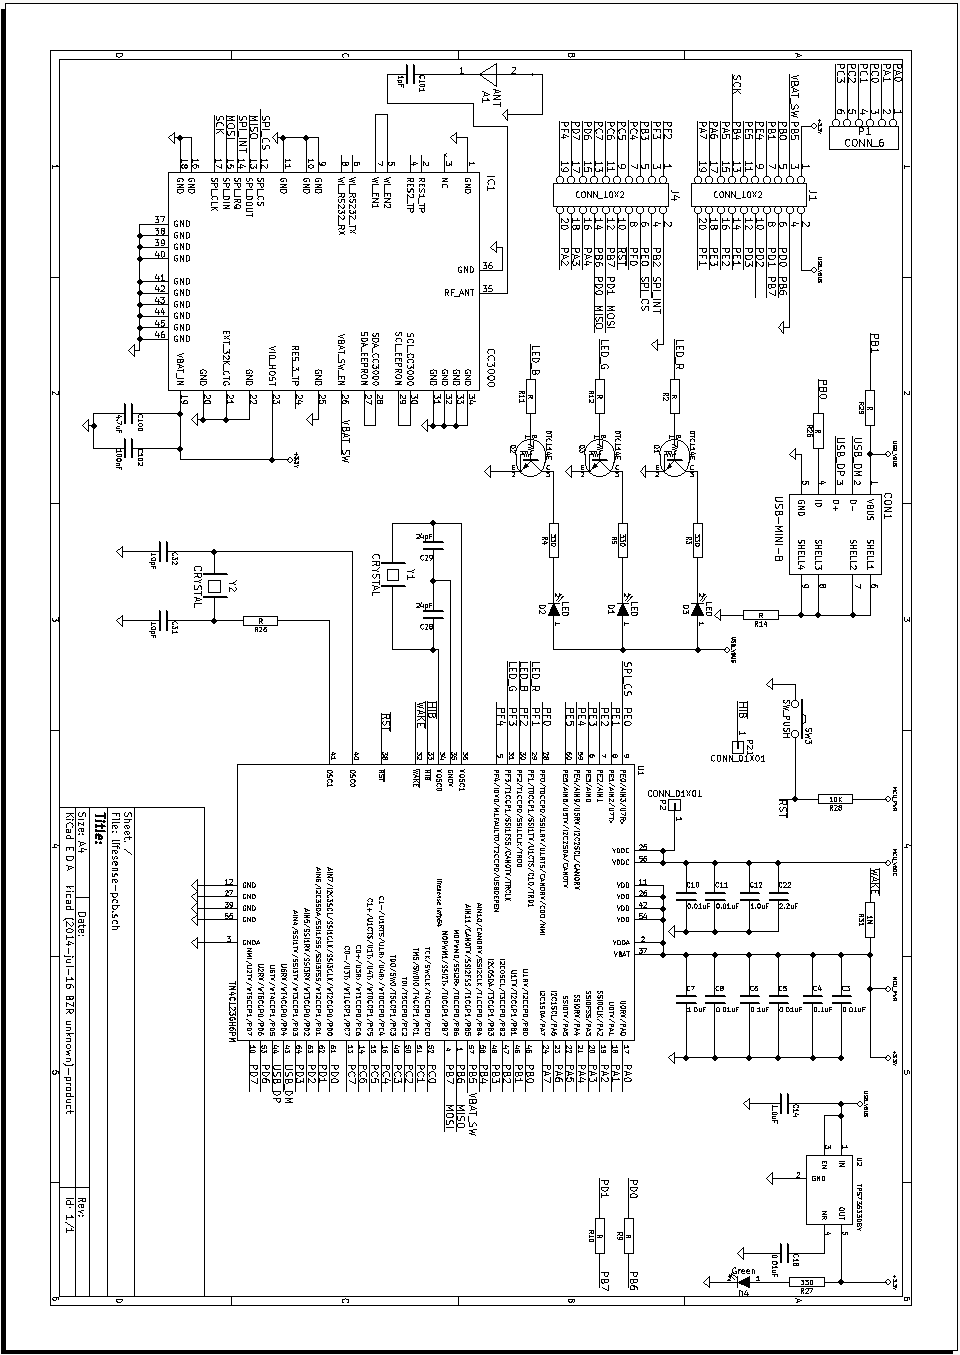
\includegraphics[width=0.8\textwidth]{schematic.png}
\caption{PCB schematic}
\end{figure}

\newpage
\section{PCB Top layer}
\begin{figure}[H]
\centering
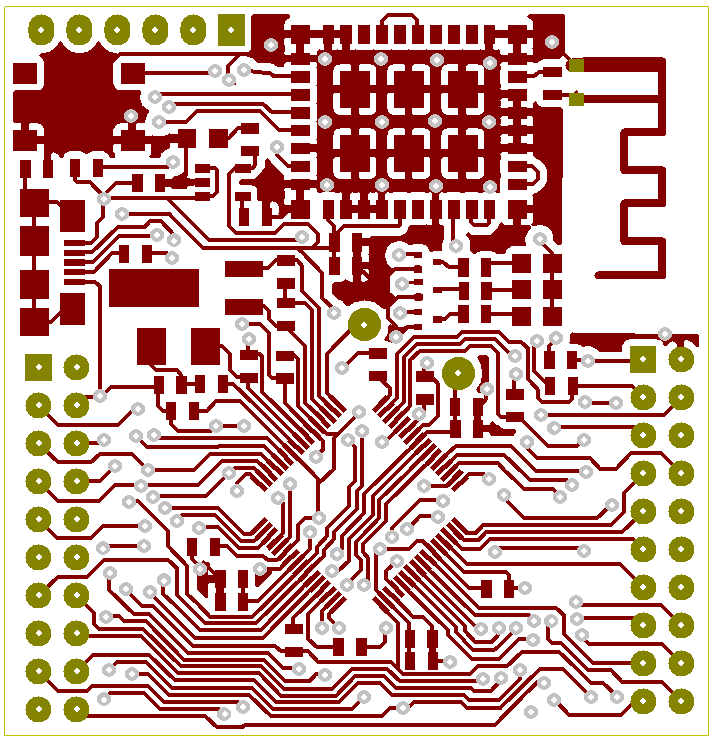
\includegraphics[width=0.9\textwidth]{front.png}
\caption{PCB Top layer}
\end{figure}

\newpage
\section{PCB Bottom layer}
\begin{figure}[H]
\centering
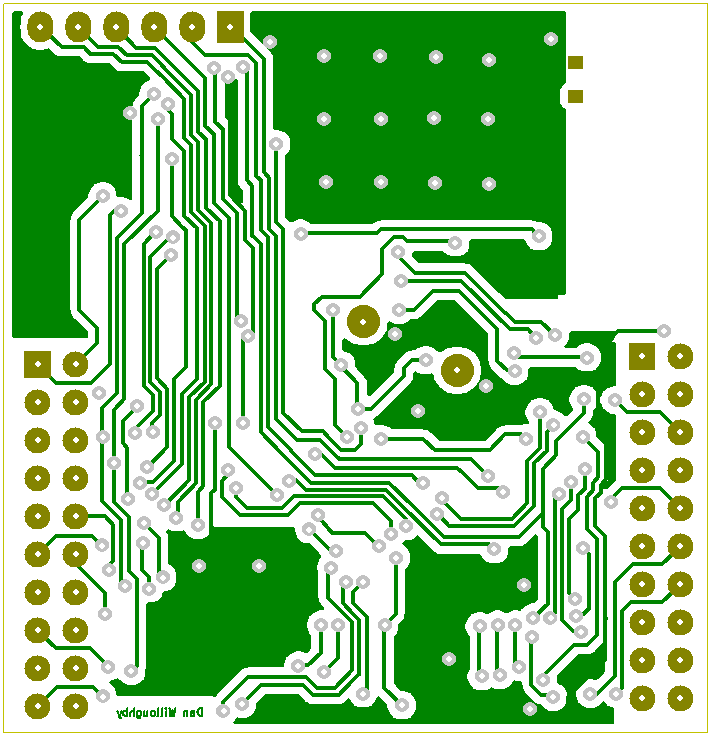
\includegraphics[width=0.9\textwidth]{back.png}
\caption{PCB Bottom layer}
\end{figure}

\newpage
\section{Poster}
\begin{figure}[H]
\centering
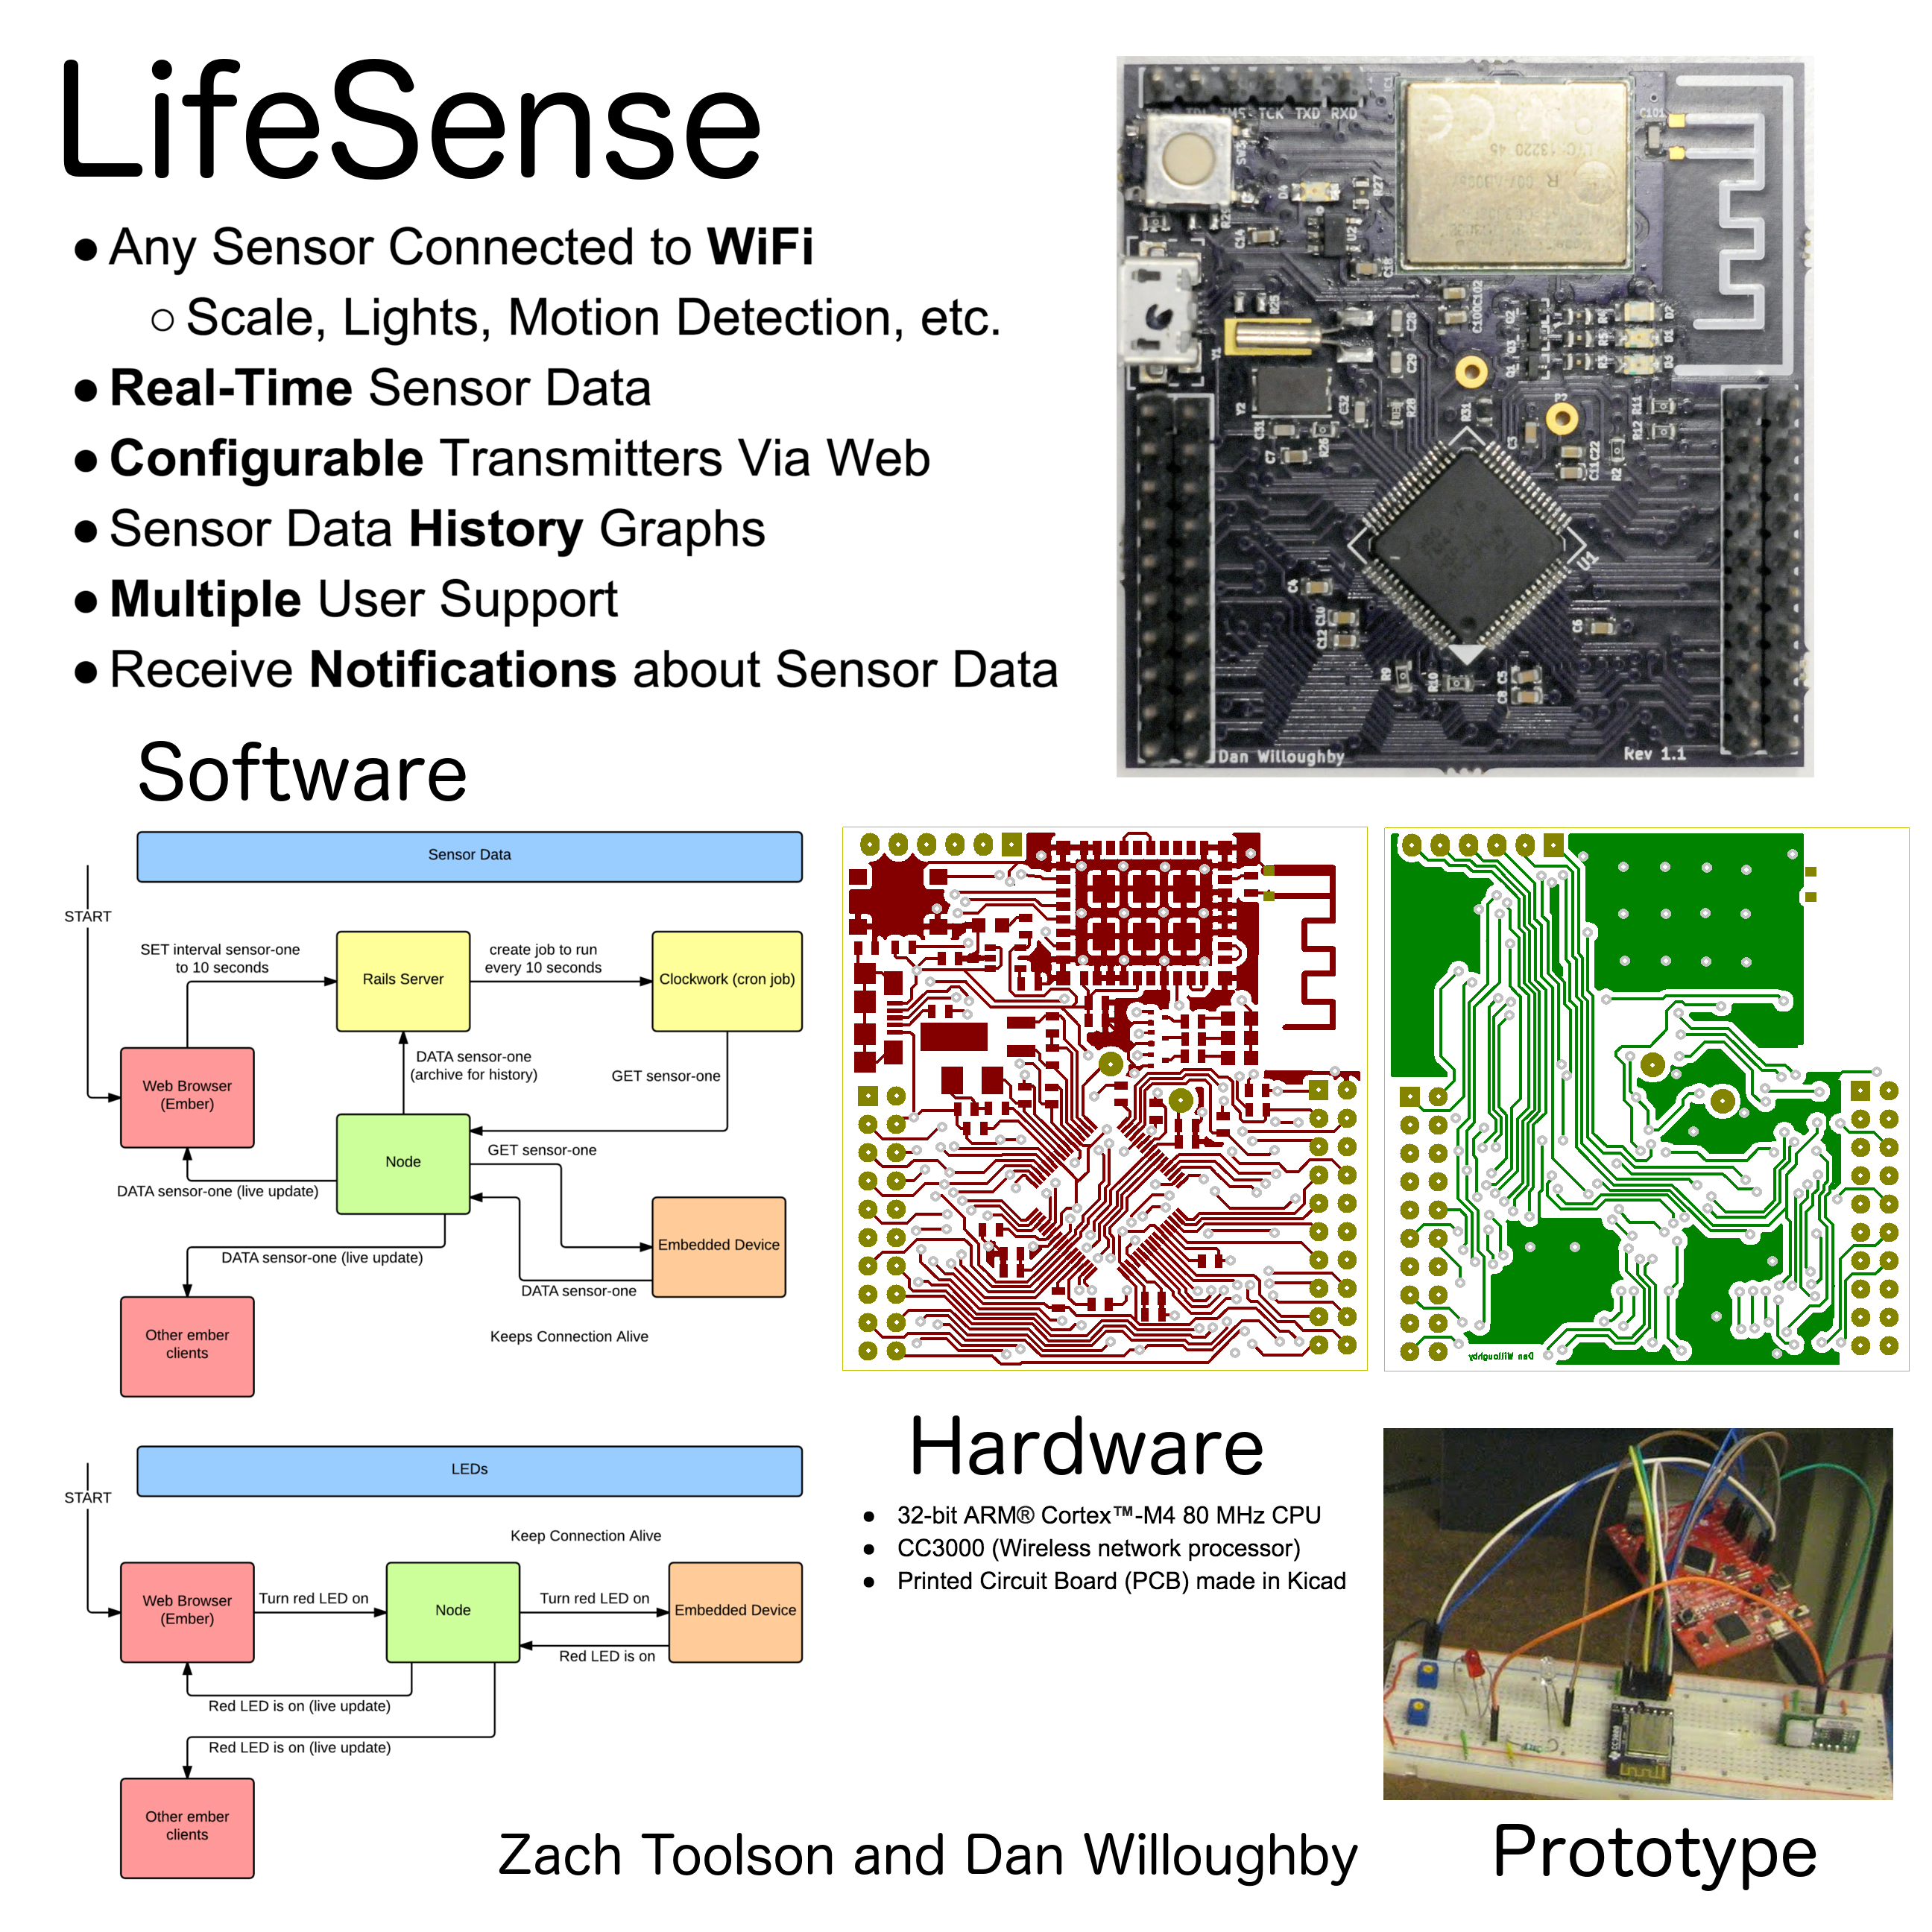
\includegraphics[width=0.9\textwidth]{poster.png}
\caption{Poster}
\end{figure}

\section{BOM}
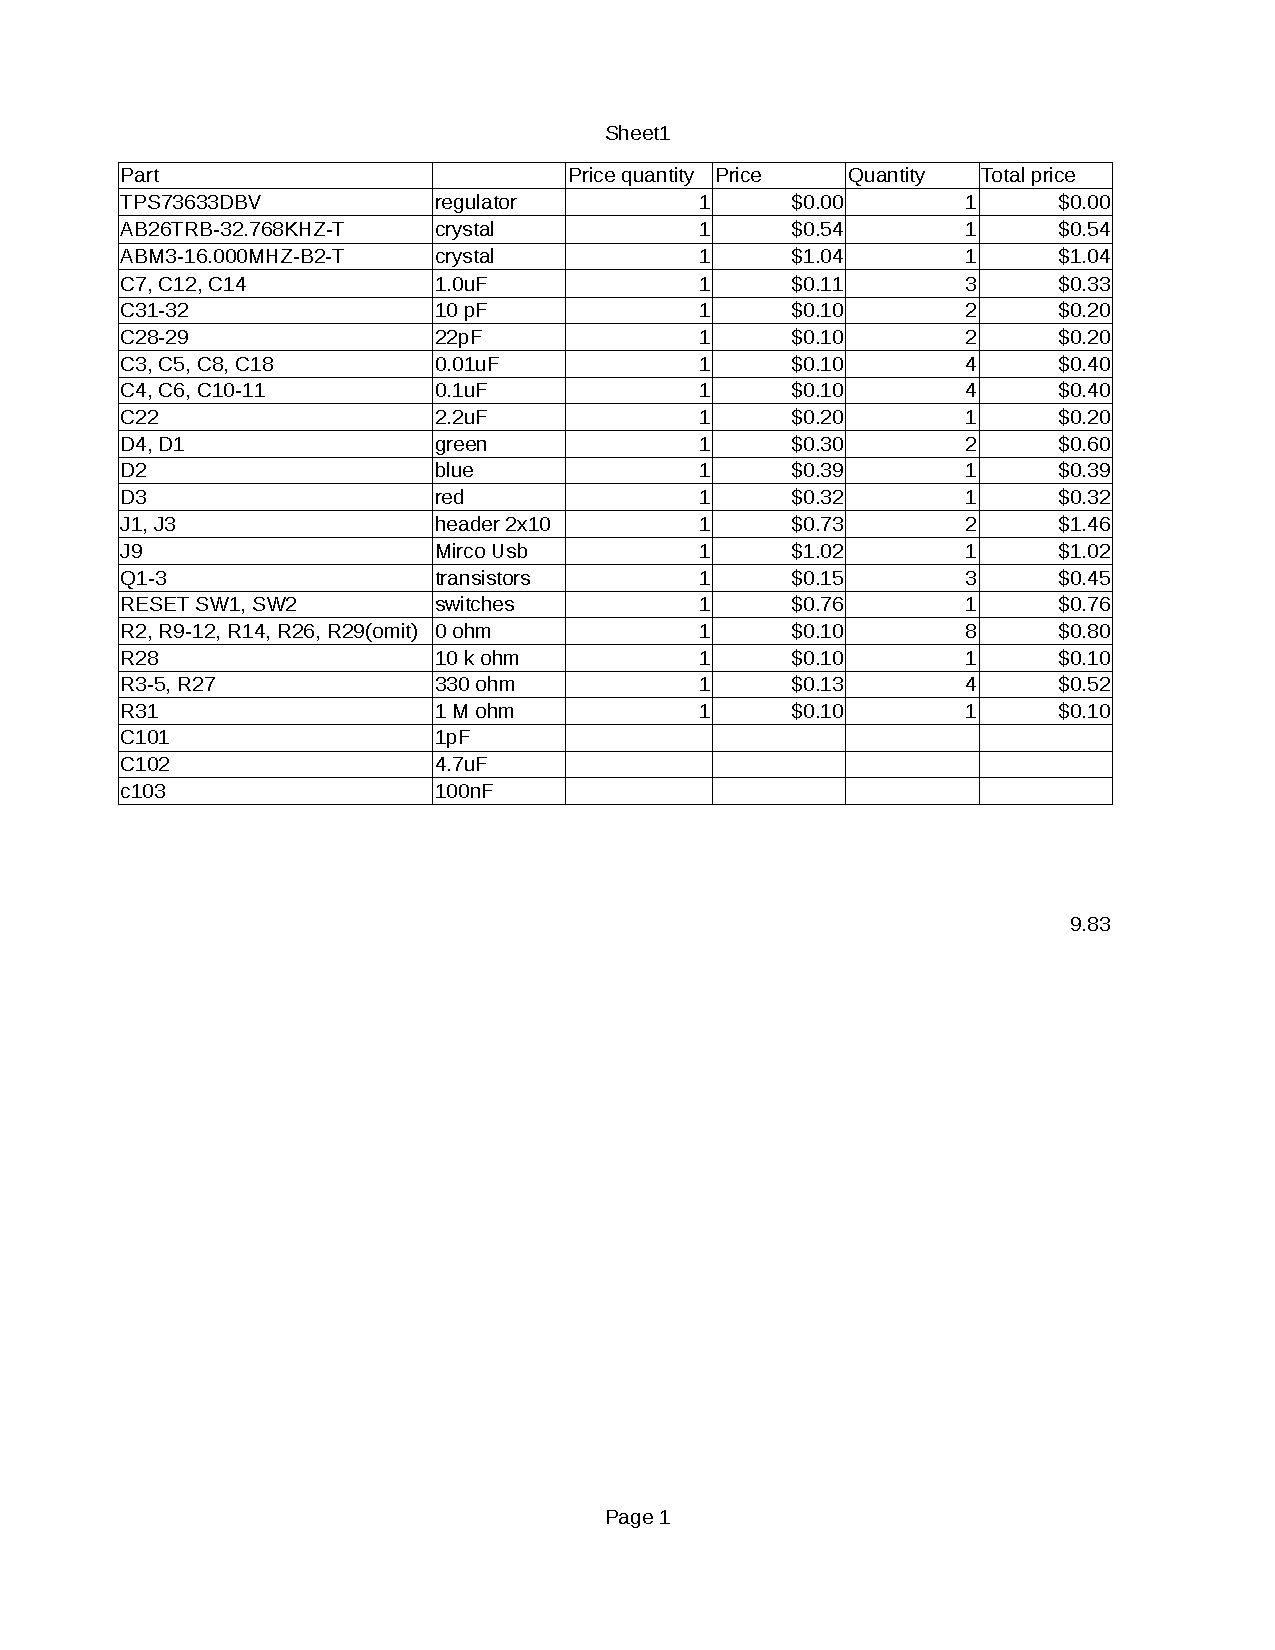
\includepdf[pages={1,2,3}]{BOM.pdf}



\end{document}
